\documentclass[tikz,border=2pt]{standalone}
\usepackage{amsmath,amssymb}
\usepackage{pgfplots}
\pgfplotsset{compat=1.18}
\usetikzlibrary{arrows.meta}

\begin{document}
% Three singularities at x = 0: removable (x^3 with the value -1 at 0, blue), jump (x^2 + 0.5 for
% x <= 0 and x + 1 for x > 0, red) and infinite (1/x, green).
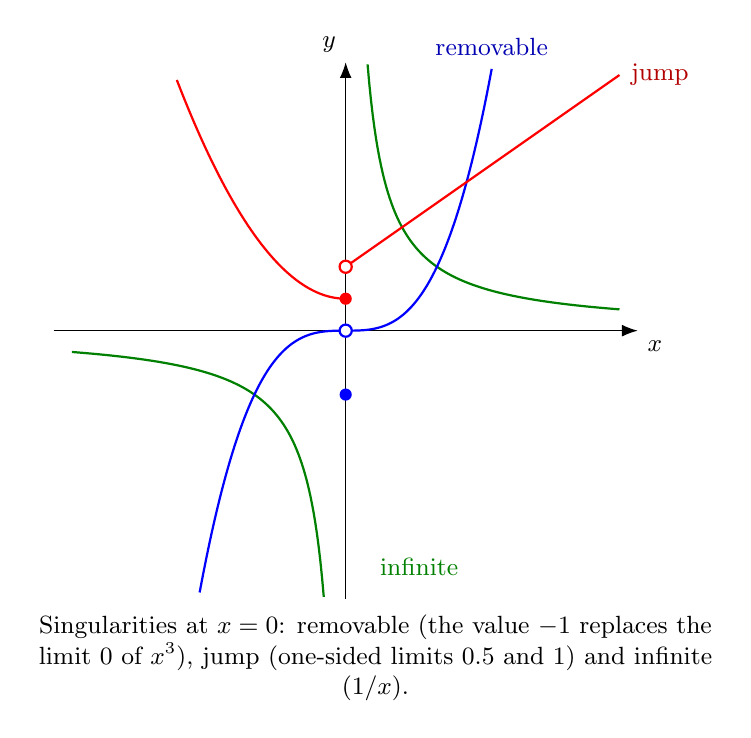
\begin{tikzpicture}[every node/.style={font=\small}]
	\begin{axis}[
		width=9cm, height=8.4cm,
		axis lines=middle, axis line style={-{Latex[length=2mm]}},
		xmin=-3.2, xmax=3.2, ymin=-4.2, ymax=4.2,
		xtick=\empty, ytick=\empty,
		tick label style={font=\small},
		xlabel={$x$}, ylabel={$y$},
		xlabel style={below right}, ylabel style={above left},
		samples=150, clip=false
		]
		\addplot[green!50!black, thick, domain=0.24:3] {1/x};
		\addplot[green!50!black, thick, domain=-3:-0.24] {1/x};
		\addplot[blue, thick, domain=-1.6:1.6] {x^3};
		\addplot[red, thick, domain=-1.85:0] {x^2+0.5};
		\addplot[red, thick, domain=0:3] {x+1};
		\draw[blue, thick, fill=white] (axis cs:0,0) circle (2.2pt);
		\fill[blue] (axis cs:0,-1) circle (2.2pt);
		\draw[red, thick, fill=white] (axis cs:0,1) circle (2.2pt);
		\fill[red] (axis cs:0,0.5) circle (2.2pt);
		\node[blue!70!black, anchor=south, font=\small] at (axis cs:1.6,4.15) {removable};
		\node[red!70!black, anchor=west, font=\small] at (axis cs:3.02,4) {jump};
		\node[green!50!black, anchor=north west, font=\small] at (axis cs:0.27,-3.4) {infinite};
	\end{axis}
	\node[anchor=north, align=flush center, text width=8.6cm] at ([yshift=-2pt]current bounding box.south) {Singularities at $x=0$: removable (the value $-1$ replaces the limit $0$ of $x^3$), jump (one-sided limits $0.5$ and $1$) and infinite ($1/x$).};
\end{tikzpicture}
\end{document}
